%% -----------------------------------------------------------------------------

\chapter{Design and Implementation}\label{ch:design}
\glsresetall % Resets all acronyms to not used

This chapter proposes a means of detecting MAC addresses through sample correlation. The algorithm is implemented in Matlab as a proof-of-concept.


%% -----------------------------------------------------------------------------

\section{High-Level Detector Design}

The high-level design of a senders detector based on MAC addresses is illustrated in figure \ref{fig:blockdesign}. From the beginning of my work until the final version, multiple design choices have changed. These and their reasons are depicted in detail in Chapter 5. The overall concept has however remained unmodified.

\begin{figure}[H]
	\centering
	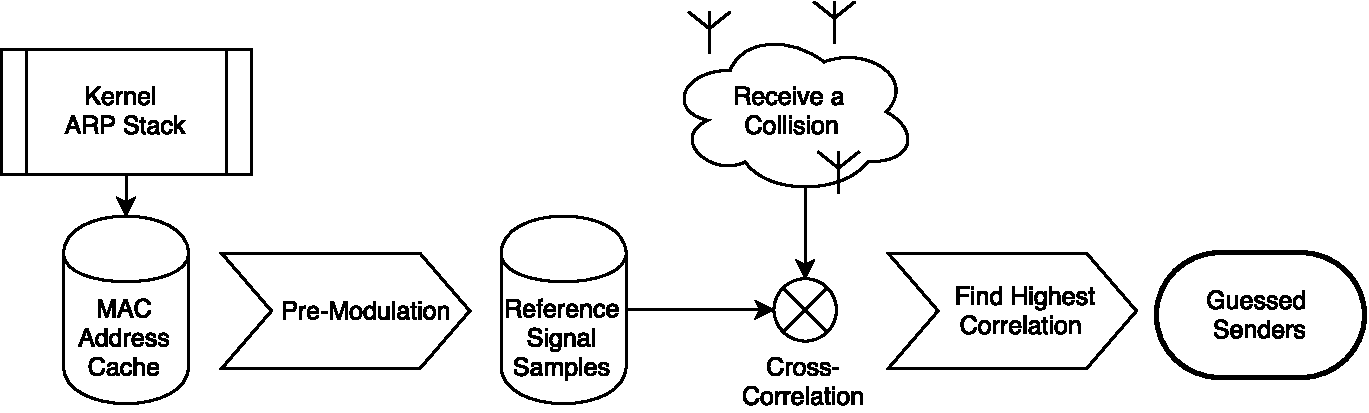
\includegraphics[width=\textwidth]{gfx/images/detector-block-design}
	\caption[High-Level Detector Design Schema]{High-Level Detector Design Schema}
	\label{fig:blockdesign}
\end{figure}

First of all, it is important to decide which MAC addresses should be tried when processing a recevied collision. Since MAC addresses are 6 byte values, there are $2^{48} \approx 3 \cdot 10^{14}$ possible instances. Although some MAC addresses are invalid, since the first three bytes denote the network interface vendor, and not all values have been issued \cite{ieeeoui}, there are still by far too many to try out all of them for every collision.

Instead, I make use of the operating system's ARP stack. During normal network operation, the kernel already keeps a cache of MAC addresses that are reachable. This list is perfectly suited for detecting senders, since it is quite likely that a collision occurs between senders that are already in the network for some time.\\

Next, I modulate IEEE 802.11 data frames for every cached MAC address. These are used as reference signals for correlation with incoming collisions. Only a small part of the reference frames contains the MAC address bits and is important for sender detection. I describe this region in detail in section \ref{sec:mac-periods}.

As mentioned in section \ref{sec:mac-and-phy}, there are different possibilities for frame modulation, namely the Modulation and Coding Scheme (MCS), the scrambler initialization, and the error-correcting convolutional encoding. Since the encoder uses a 7 bit state, only the MAC header field directly preceeding the sender MAC address is relevant here. That field is the destination MAC address. In theory, all possible combinations could be modulated for the refernce signals cache, however this would mean a total amount of  more than 130 thousand candidates for every MAC address in the ARP pool. In chapter \ref{ch:evaluation} I evaluate which fields matter to which extent.

$$ N_{MCS} \cdot N_{Scrambler} \cdot N_{Dest} = 8 \cdot 127 \cdot 128 = 130 048 $$\vspace{0cm}

The modulation process comprises the following steps:

\begin{enumerate}
	\item Generate a MAC header with appropriate sender and destination MAC addresses
	\item Apply the scrambler with specific initialization value
	\item Run the convolutional encoder, which is deterministic
	\item Group bits and interleave symbols
	\item For a time-domain signal, apply inverse fourier transform and add a cyclic prefix
\end{enumerate}

For correlation in the frequency-domain, I omit step 5. The received collision signal has to be applied to the fourier transform in this case. I have done experiments with frequency-domain detection and show the results of these in section \ref{sec:freqd-correlation}.\\

When the receiver senses a transmission, I determine whether it is a collision using the IEEE 802.11 Long Training Field. Section \ref{preamble-corr} gives details about this process. This also yields a possible delay between the two frames.

Upon noticing a collision, all reference samples are correlated with the signal under test. The correlations are then sorted descending by correlation magnitue.

\begin{itemize}
	\item There should be four peaks, indicating sender and receiver of both packets
	\item symbol modulation -> do 6 bytes of address data provide enough samples to correlate to? With 64-QAM?
	\item convolutional encoding, puncturing, and interleaving deterministic?
\end{itemize}

%% -----------------------------------------------------------------------------

\section{Detecting Frames and Collisions}\label{sec:preamble-corr}


%% -----------------------------------------------------------------------------

\section{Periods containing MAC Addresses}\label{sec:mac-periods}


%% -----------------------------------------------------------------------------

\section{Matlab Implementation}
